\section{Dashboard mit Kennzahlen des Netzmodells}
\label{chp:dashboard}

\setcapindent{0pt}
\begin{wrapfigure}{r}{0.27\textwidth}
  \begin{center}
    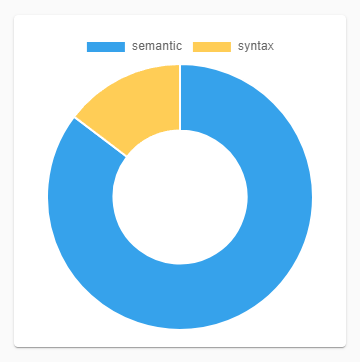
\includegraphics[width=0.8\linewidth]{content/img/Empire/Frontend/Dashboard_Donatdiagramm.png}
  \end{center}
  \caption{Donatdiagramm}
  \label{fig:einfachesDonatdiagramm}
\end{wrapfigure}
\setcapindent{83pt}

Kennzahlen in einem Dashboard attraktiv, benutzerfreundlich und intuitiv darzustellen, ist selbst für fortgeschrittene Designer oft ein langwieriger Prozess. Eine einfache Art, die Dauer für die Schaffung eines übersichtlichen Dashboardes zu minimieren, ist die Verwendung von vorgefertigten UI-Elementen. Diese Elemente können aus beliebigen Bibliotheken stammen. Für Angular eignet sich am besten die Bibliothek \emph{ng2-charts}.

In der Abbildung \ref{fig:einfachesDonatdiagramm} rechts ist ein Beispiel eines Donatdiagrammes mittels ng2-charts gegeben. Dieses wird im Dashboard verwendet, um die Verteilung der beiden Kategorien darzustellen.

Die Bibliothek ng2-charts ist im Prinzip eine Schnittstelle zwischen Angular und einer universellen Javascript-Diagramm-Bibliothek namens \emph{Chart.js}. Diese unterstützt wiederum eine Vielzahl an Diagrammen, von Linien- über Flächen bis hin zu Donatdiagrammen. Für das Dashboard unseres Netzwerkanalyseprogrammes habe ich ausschließlich Donatdiagramme verwendet, um die prozentuellen Verteilungen der verschiedenen Eigenschaften, darunter der Schweregrad, die Kategorie, das Spannungslevel und die Klasse beziehungsweise der Typ des Fehlers, einheitlich darzustellen. \cite{ng2-charts}

Diese Bibliothek wird nun verwendet, um vier Donatdiagramme auf dem Dashboard darzustellen. Diese Diagramme geben den Ingenieuren von Siemens einen schnellen Überblick über grundlegende Eigenschaften der aktuellen Fehler im Netzmodell. Jedes der vier Diagramme stellt die prozentuelle Verteilung bezüglich einer Eigenschaft dar. Diese vier Eigenschaften sind: Klasse, Kategorie, Schweregrad und Spannungslevel. Wie Sie in Abbildung \ref{fig:PrototypeDashboard} sehen können, sind alle vier Eigenschaften sehr einseitig. Mit dieser Einseitigkeit ist die klare Dominanz beziehungsweise die Vorherrschaft des Hauptsegmentes der jeweiligen Eigenschaft gemeint. An den Legenden können Sie sehen, dass beispielsweise fast alle Fehler im Netzmodell mit Schweregrad \wordindoublequotes{CRITICAL} kategorisiert worden sind (der große gelbe Anteil im dritten Diagramm in Abbildung \ref{fig:PrototypeDashboard}).

\begin{figure}
    \centering
    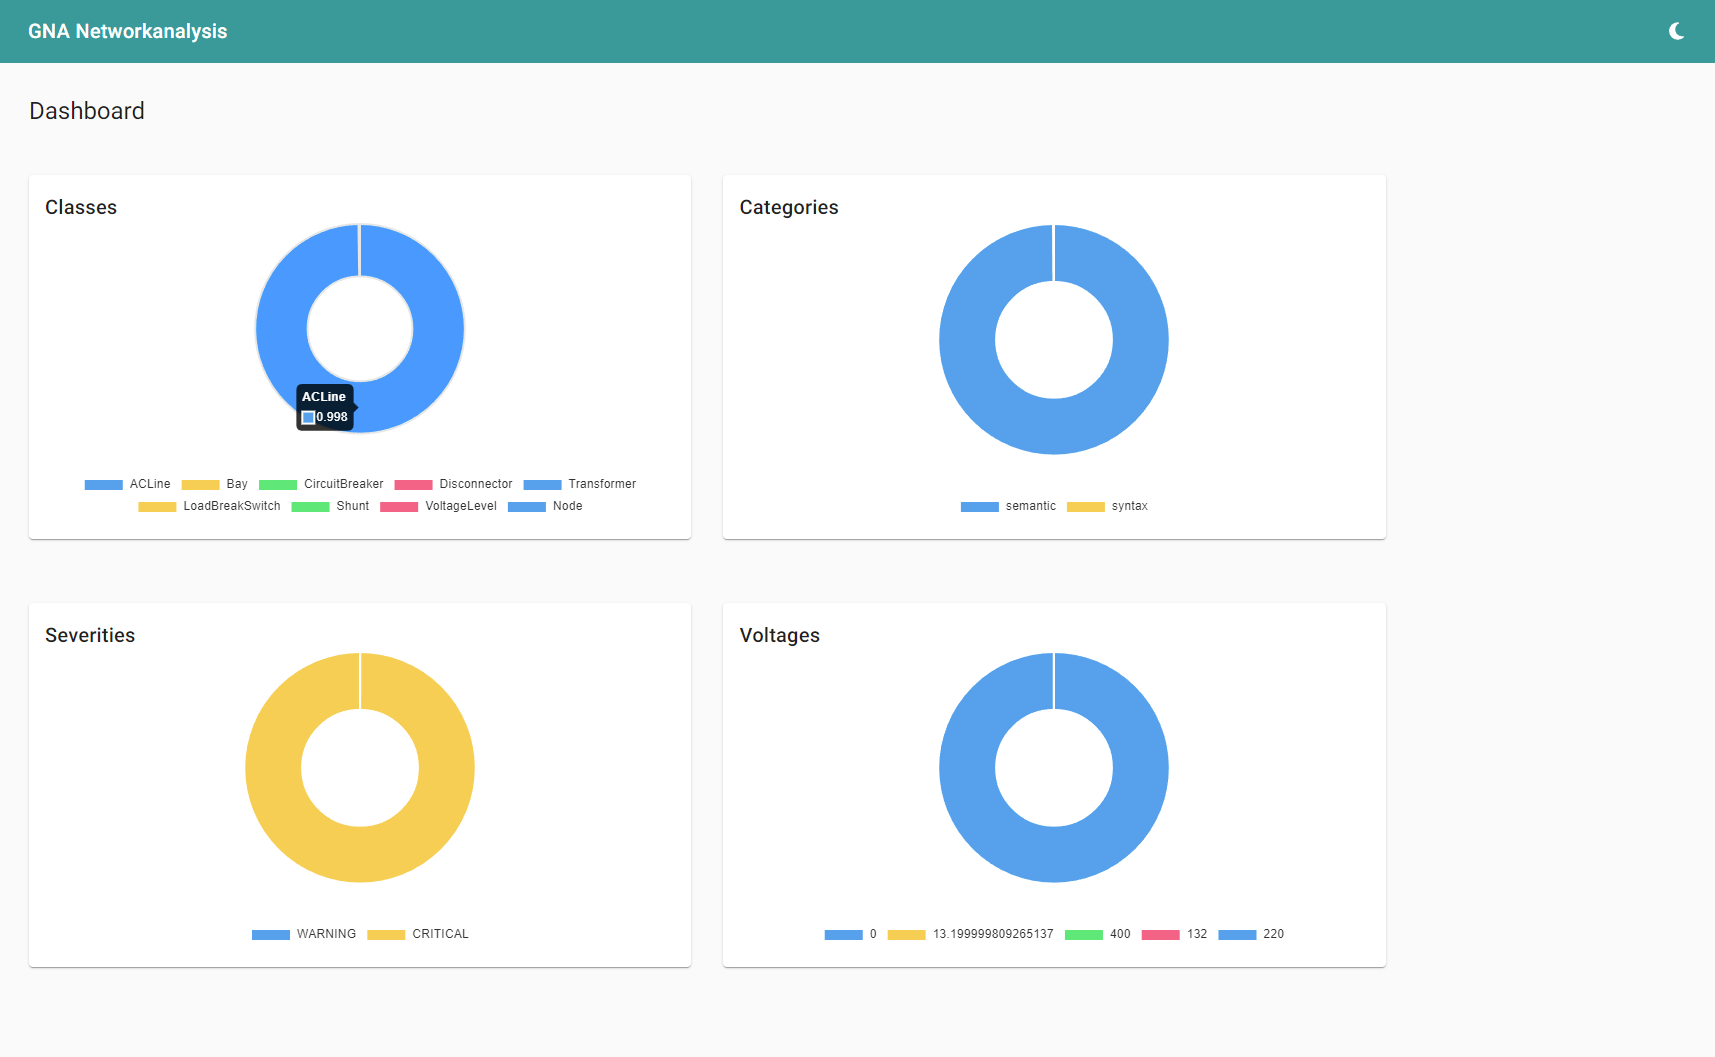
\includegraphics[width=1\textwidth]{content/img/Empire/Frontend/Angular_Dashboard_Prototype.png}
    \caption{Dashboard des Prototypen}
    \label{fig:PrototypeDashboard}
\end{figure}
\FloatBarrier

Bei diesen Diagrammen wird auch ein hoher Wert auf die Interaktivität gelegt. Wie Sie beim ersten Diagramm in Abbildung \ref{fig:PrototypeDashboard} auch sehen können, gibt es eine dem Mauszeiger folgende Informationen bezüglich des Anteils dieses ausgewählten Segments. Dieser sogenannte \wordindoublequotes{Tooltip} ist äußerst intuitiv, da er heutzutage schon an vielen Stellen in der Webentwicklung auftritt. \cite{chartjs-interactions}

Um die Interaktivität noch mehr zu steigern, ist bei Chart.js standardmäßig auch die Funktion implementiert, bestimmte Anteile im Diagramm dynamisch auszublenden. Bei schlauem Anwenden dieser Funktion, können bereits sehr nützliche Informationen aus einigen Diagrammen abgelesen werden, wie Sie in Abbildung \ref{fig:PrototypeDashboardInteraction} sehen. Sie sehen zum Beispiel, dass ein Großteil der gefilterten Fehler bei Stromkreisunterbrechern und Knoten entsteht (Diagramm 1) und nur sehr wenige Fehler eine Spannung von 400V aufweisen. \cite{chartjs-legend}

\begin{figure}
    \centering
    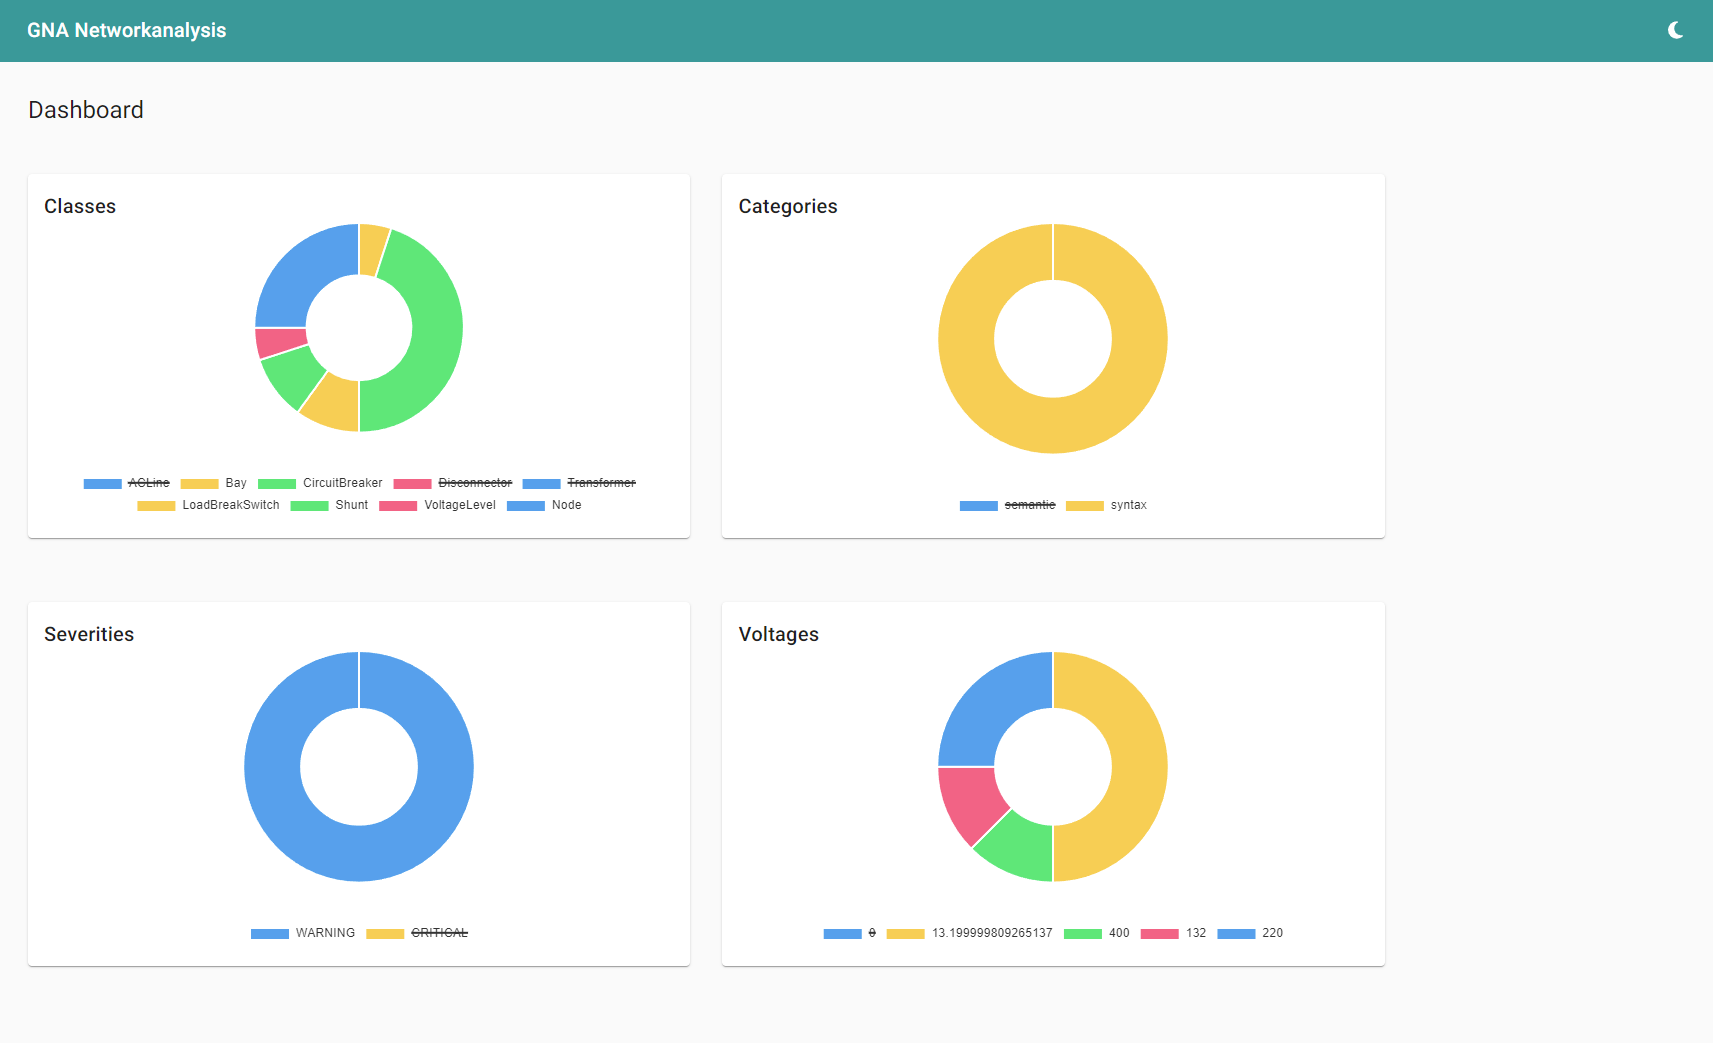
\includegraphics[width=1\textwidth]{content/img/Empire/Frontend/Angular_Dashboard_Interaction_Prototype.png}
    \caption{Interaktion mit den Diagrammen des Dashboardes}
    \label{fig:PrototypeDashboardInteraction}
\end{figure}
\FloatBarrier

Summa summarum ist das Dashboard ein sehr effizienter Weg, um einen schnellen Überblick über das aktuelle Geschehen im Netzmodell zu erhalten und bestimmte Eigenschaften im allgemeinen Kontext zu interpretieren. Die Diagramme sind intuitiv zu lesen und mit einigen Interaktionen ausgestattet. Außerdem ist das Dashboard eine wichtige Komponente moderner Applikationen, da diese immer eine Art Landingpage beziehungsweise Einstiegsseite für die Benutzer ist und diesen herzlich willkommen heißt.